\documentclass{report}
\usepackage[fontsize=13pt]{scrextend}

\usepackage{my_lab}

\begin{document}

\graphicspath{{figures}}

\LabTitle{3.7.1}{Скин-эффект}

\begin{document}
\textbf{Цель работы:} Исследование проникновения переменного магнитного поля в медный полый цилиндр

\section*{Теоретическая часть}
\subsection*{Скин-эффект для полупрастранства}
\begin{wrapfigure}{l}{0.3\textwidth}
	\centering
	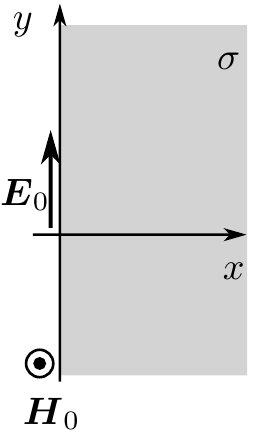
\includegraphics[width=0.28\textwidth]{poluprostranstvo}
	%\caption{Скин-эффект в полупространстве}\label{fig:poluprostranstvo}
\end{wrapfigure}

Рассмотрим квазистационарное поле внутри проводящей среды в простейшем плоском случае.
Пусть вектор $\vb*{E}$ направлен всюду вдоль оси $y$ и зависит только от координаты $x$, т. е. ${E_x} = {E_z} \equiv 0$, $E_y=E_y(x,t)$.
В квазистационарном приближении
\begin{equation*}
	\grad \times \vb*{H} = \sigma \vb*{E}
\end{equation*}

Преобразуя это уравнение, можно получить уравнение, схожее с уравнением диффузии:
\begin{equation}
	\grad^2\vb*{H}=\sigma\mu\mu_0 \frac{\partial \vb*{H}}{\partial t}\label{eq:laplacian_H}
\end{equation}
Точно такое же уравнение имеет место и для вектора $E:$
\begin{equation}
	\grad^2\vb*{E}=\sigma\mu\mu_0 \frac{\partial \vb*{E}}{\partial t}\label{eq:diffusion}
\end{equation}

Подставляем в (\ref{eq:diffusion}) наше электрическое поле $E_y=E_y(x,t)$
\begin{equation}
	\frac{\partial^2 E_y}{\partial x^2} = \sigma\mu\mu_0\frac{\partial E_y}{\partial t}
	\label{eq:diffusion_chastni}
\end{equation}
Если $E_y(0,t)=E_0 e^{i\omega t}$ то решением (\ref{eq:diffusion_chastni}) будет функция вида
\begin{equation}
	E_y(x,t)=E_0 e^{-x/\delta} e^{i(\omega t - x/\delta)}
	\label{eq:skin_effect_poluprostranstvo}
\end{equation}
где
\begin{equation}
	\delta = \sqrt{\frac{2}{\omega\sigma\mu\mu_0}}
	\label{eq:delta}
\end{equation}

\newpage
\subsection*{Скин-эффект в тонокм полом цилиндре}
\vspace{1cm}
\begin{wrapfigure}[36]{l}{0.3\textwidth}
	\begin{center}
		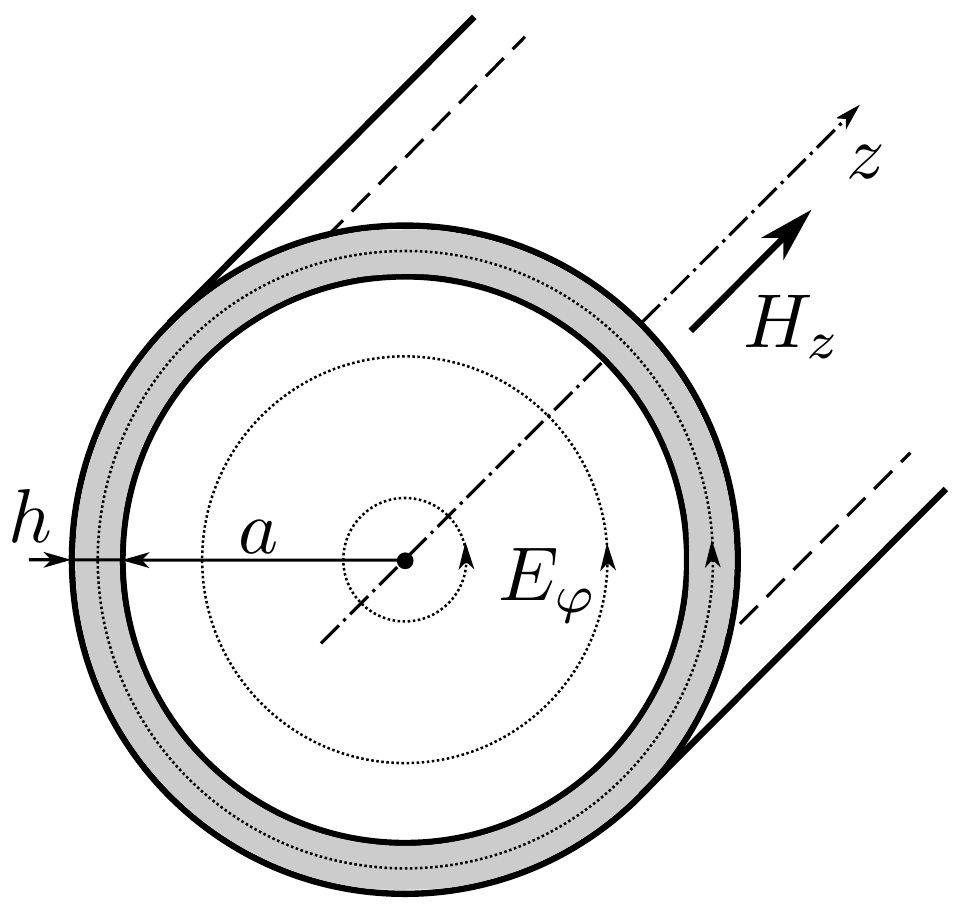
\includegraphics[width=0.28\textwidth]{cilindr}
	\end{center}
	\caption{Эл-магнитные поля в цилиндре}\label{fig:cilindr}

	\begin{center}
		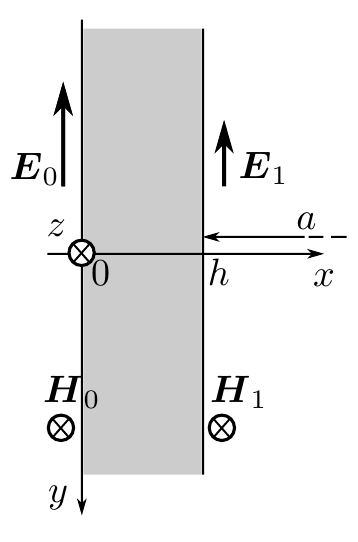
\includegraphics[width=0.28\textwidth]{stenka}
	\end{center}
	\caption{Стенка цилиндра}\label{fig:stenka}
\end{wrapfigure}

Перейдем теперь к описанию теории в нашей работе. Из соображении симметрии и
непрерывности соответствующих компонет векторов $\vb*{E}$ и $\vb*{H}$ можем сказать что
\begin{equation*}
	H_z = H(r)e^{i\omega t} \text{, } E_\varphi = E(r)e^{i\omega t}
\end{equation*}
и при этом функции $H(r)$ и $E(r)$ непрерывны.

Внутри цилиндра токов нет, следовательно $H(r)=H_1=\text{const}$ внутри цилиндра.
По теореме об электромагнитной индукции
\begin{equation*}
	E(r) = -\frac{1}{2}\mu_0 r \cdot i \omega H_1
\end{equation*}
откуда мы получаем граничное условие
\begin{equation}
	E_1=E(a)= -\frac{1}{2}\mu_0 a \cdot i \omega H_1
	\label{eq:granichnoe_uslovie_E}
\end{equation}

В прближении $h \ll a$ можем пренебречь кривизной стенки и смоделировать
его бесконечной полосой. Тогда, надо решить уравнение (\ref{eq:laplacian_H})
с граничными условиями. Решая уравнение получим связь полей $H_1$
(поле внутри цилиндра которое мы будем измерять) и $H_0$, которое колебается с частотой
$\omega$

\begin{equation}
	H_1 = \frac{H_0}{\ch(\alpha h) + \frac{1}{2} \alpha a \sh(\alpha h)}
	\text{\ \ \ }
	\alpha = \sqrt{i\omega \sigma \mu_0} = \frac{\sqrt{2}}{\delta}e^{i\pi/4}
	\label{eq:svyaz_poley}
\end{equation}

из этой формулы получим сколько по фазе отстает поле $H_1$ от $H_0$. При $\delta \ll h$
(высокачастотная область)

\begin{equation}
	\psi \approx \frac{\pi}{4} + \frac{h}{\delta} =
	\frac{\pi}{4} + h \sqrt{\frac{\omega \sigma \mu_0}{2}}
	\label{eq:faza_high_freq}
\end{equation}

При $\delta \gg h$ (низкочастотная область)

\begin{equation}
	\tg \psi \approx \frac{ah}{\delta^2} = \pi a h \sigma \mu \mu_0 \nu
	\label{eq:faza_low_freq}
\end{equation}

\subsection*{Установка и процесс измерения}
\begin{wrapfigure}{l}{0.4\textwidth}
	\begin{center}
		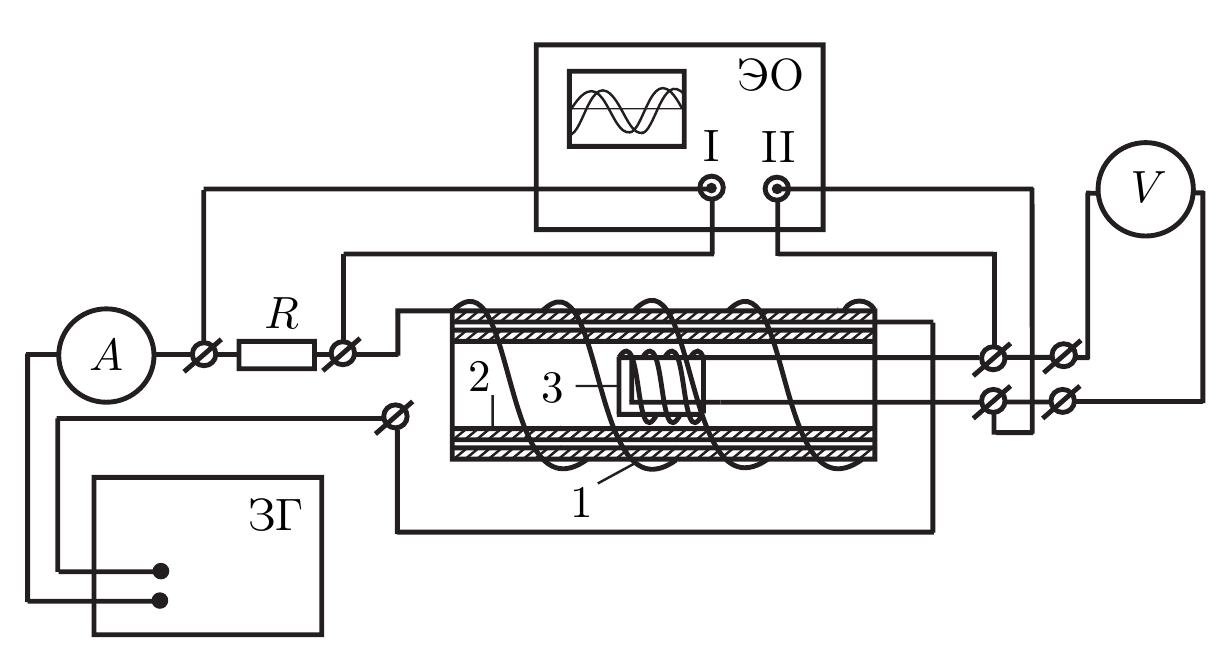
\includegraphics[width=0.38\textwidth]{ustanovka}
	\end{center}
	\caption{Установка}\label{fig:ustanovka}
\end{wrapfigure}

Переменное магнитное поле создается соленоидом 1, на который подается переменный ток со звукового генератора ЗГ. Внутри соленоида расположен медный экран 2. Магнитное поле внутри цилиндра измеряется катушкой 3. Напряжение на катушке пропорциональна производной $\dot{B_1}(t)$
\begin{equation*}
	U(t) \propto \dot{B_1}(t) = -i\omega H_1 e^{i\omega t}
\end{equation*}
Поле внутри цилиндра пропорциональна току через соленоид
\begin{equation*}
	H_0(t) \propto I(t)
\end{equation*}
Отсюда несложно увидеть, что
\begin{equation}
	\frac{\abs{H_1}}{\abs{H_0}} = c \cdot \frac{U}{\nu I} = \xi_0 \xi
	\label{eq:otnoshenie_amplitud}
\end{equation}
где константу  $\xi_0$ можно определить из условия $\abs{H_1}/\abs{H_0} \rightarrow 1$ при
$\nu \rightarrow 0$.\\

При измерениях разности фаз нужно учесть, что первый сигнал на осциллографе
пропорционален магнитному полю снаружи, а второй пропорционален производному
поля внутри цилиндра по времени, поэтому измеренная на осциллографе разность фаз $\varphi$ будет на $\frac{\pi}{2}$ больше реальной $\psi$:
\[\varphi = \psi + \frac{\pi}{2}\]

\section{Ход работы}
Параметры установки: $$2a = 45 \mm$$ $$h=1.5 \mm$$
Проводимость: $$\sigma \sim 5\cdot 10^7 \Cm / \m$$
Получаем оценку для частоты, при которой
глубина проникновения равна толщине стенок цилиндра: $$\nu_h = 2254\ \Hz$$

\subsection{Измерения амплитуд в области низких частот}
В области частот $\nu \ll \nu_h$ $\alpha h \ll 1$, и из (\ref{eq:svyaz_poley}) получаем
\begin{equation*}
	\frac{1}{\xi^2}=\xi_0^2B^2\nu^2 + \xi_0^2,
    \quad B=\pi a h \sigma \mu_0
	\label{eq:liniya_dlya_c}
\end{equation*}

\begin{figure}[H]
	\centering
	\includesvg[width=0.9\linewidth]{figures/graph1.svg}
	\caption{График зависимости $1/\xi^2(\nu^2)$}\label{fig:xi_nu_low_freq_linearized}
\end{figure}

\begin{table}[H]
	\centering
	\begin{tabular}{|l|l|l|}
        \hline
		$\nu, \Hz$ & $I, A$ & $U, \Volt$ \\
        \hline
		25         & 473.18 & 162.1      \\
		30         & 471.12 & 192.8      \\
		35         & 468.87 & 222.6      \\
		40         & 466.29 & 251.4      \\
		45         & 463.4  & 279.1      \\
		50         & 460.4  & 305.7      \\
		55         & 457.27 & 331.2      \\
		60         & 453.88 & 355.2      \\
		65         & 450.47 & 378.5      \\
		70         & 447.07 & 400.5      \\
		75         & 443.56 & 421.3      \\
		80         & 440.07 & 441        \\
		85         & 436.63 & 459.5      \\
		90         & 433.2  & 477.1      \\
		95         & 429.84 & 493.5      \\
		100        & 426.5  & 509        \\
		105        & 423.24 & 523.6      \\
		110        & 420.08 & 537.2      \\
		115        & 417    & 550.1      \\
        \hline
	\end{tabular}
    \hspace{1cm}
	\begin{tabular}{|l|l|}
        \hline
		$\nu^2, \Hz^2$ & $\frac{1}{\xi^2}, A$ \\
        \hline
		5326       & 625    \\
		5374       & 900    \\
		5435       & 1225   \\
		5504       & 1600   \\
		5582       & 2025   \\
		5670       & 2500   \\
		5766       & 3025   \\
		5878       & 3600   \\
		5984       & 4225   \\
		6106       & 4900   \\
		6235       & 5625   \\
		6373       & 6400   \\
		6524       & 7225   \\
		6678       & 8100   \\
		6847       & 9025   \\
		7021       & 10000  \\
		7204       & 11025  \\
		7399       & 12100  \\
		7599       & 13225  \\
        \hline
	\end{tabular}
\end{table}

Получаем следующие значения:
\begin{gather*}
\alpha = \dv{x}{y} \approx 0.18 \frac{1}{\Ohm^2} \\
\beta = y(0) \approx 5200 \frac{\Hz^2}{\Ohm^2}
\end{gather*}
\begin{gather*}
\xi_0 \approx 72 \frac{\Hz}{\Ohm} \\
\sigma \approx (4.51 \pm 0.01) 10^7 \frac{\Cm}{\m}
\end{gather*}

\subsection{Измерение проводимости через разность фаз в низкочастотном диапазоне}
Согласно формуле (\ref{eq:faza_low_freq}), при $\delta \gg h$
\begin{equation*}
    \tan \psi = k \cdot \nu, \quad k = \pi a h \sigma \mu_0 \ \ (\mu = 1)
\end{equation*}

\begin{figure}[H]
    \centering
    \includesvg[width=0.9\linewidth]{figures/graph2.svg}
\end{figure}

Из коэффициента наклона прямой находим проводимость
\begin{equation}
    \sigma = (4.7 \pm 0.2) \cdot 10^7 \Cm/\m
\end{equation}

\subsection{Измерение проводимости через разность фаз в высокачастотном диапазоне}
$$
\psi - \frac{\pi}{4} = \alpha \sqrt{\nu}, \quad \alpha = h \sqrt{\pi \mu_0 \sigma}
$$
\begin{figure}[H]
    \centering
    \includesvg[width=0.9\linewidth]{figures/graph3.svg}
\end{figure}

\begin{equation}
    \sigma = (4.4 \pm 0.3) \cdot 10^7 \Cm/\m
\end{equation}

\subsection{Измерение проводимости через изменение индуктивности}
\begin{equation*}
    \frac{L_{\max} - L}{L - L_{\min}} = K \nu^2, \quad K = \pi ^2 a^2 h^2 {\mu_0}^2 \sigma^2
\end{equation*}

\begin{figure}[H]
    \centering
    \includesvg[width=0.9\linewidth]{figures/graph4.svg}
\end{figure}
\begin{figure}[H]
    \centering
    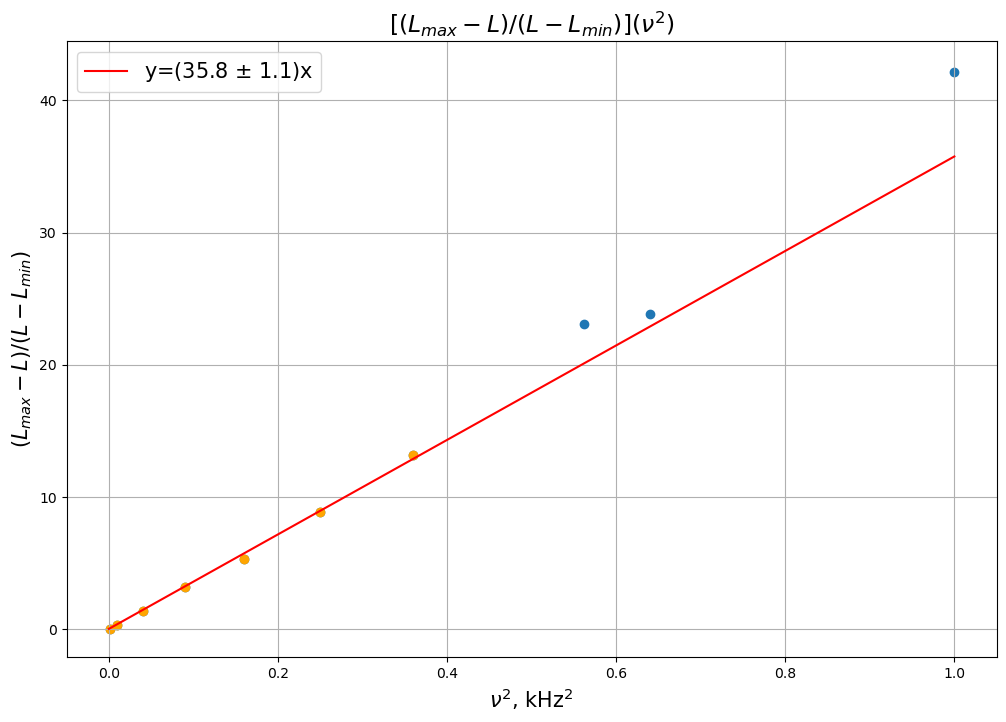
\includegraphics[width=0.9\linewidth]{figures/graph5.png}
\end{figure}
\begin{equation}
    \sigma = (4.5 \pm 0.1) \cdot 10^7 \Cm/\m
\end{equation}

\subsection{Отношение магнитных полей}
Найдем $\abs{H_1}/\abs{H_0}$ двумя способами - через
формулу (\ref{eq:otnoshenie_amplitud}) и (\ref{eq:svyaz_poley}).

\begin{figure}[H]
    \centering
    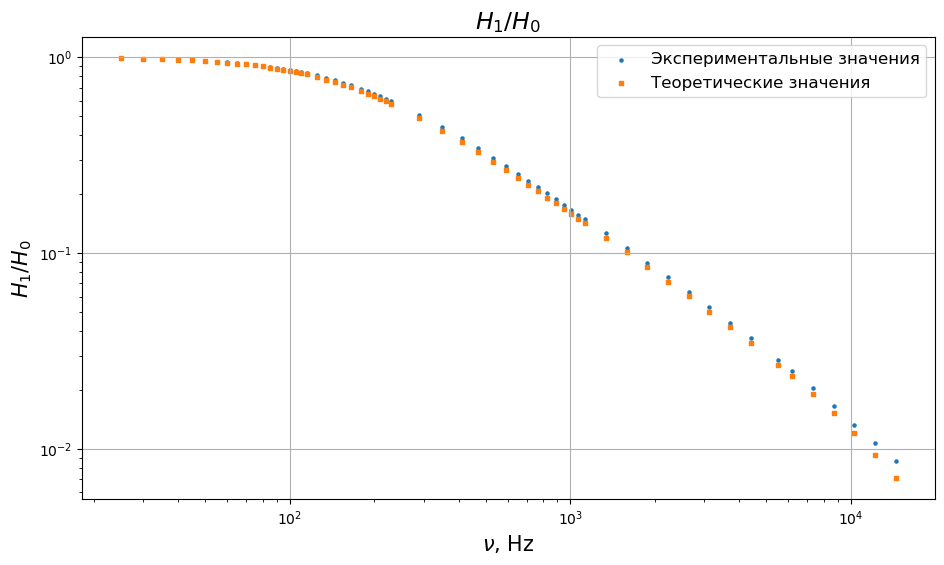
\includegraphics[width=0.9\linewidth]{figures/graph6.png}
\end{figure}

\section{Выводы}
В данной лабораторной работе мы измеряли удельную проводимость меди 4-мя
различными способами с помощью явления скин-эффекта. \\
\begin{equation}
    \sigma_\text{табл} \approx 5.6 \cdot 10^7 \Cm/\m
\end{equation}
В целом, наши измерения заметно меньше истинного. \\
Меньше всего получилась погрешность измерения на низких частотах. \\
На высоких частотах, скорее всего, измерениям мешают токи Фуко. \\
Также посчитали отношение магнитных полей. Значения хорошо совпали с
теоретическими значениями.
\end{document}
